\section{Introduction}

A cellular automaton is a grid of cells, each in one of a few states, that evolves in discrete
time: at every step, every cell simultaneously takes a new state computed from the states of its
neighbors by a fixed local rule. The interest of the model lies in the contrast between the
simplicity of the rules and the richness of what they produce: a three-cell rule draws the
Sierpi\'nski triangle, and Conway's Game of Life is capable of universal computation.

The goal of the project is \emph{not} to program one such automaton. It is to design an
architecture able to simulate \emph{any} automaton described in an input file: a grid whose
number of dimensions is only known at run time, neighborhoods that may be predefined or declared
by the user, and an evolution rule written in a small language of nested operators.

This report presents \textbf{Cellula}, the application written to that end. It is a Java~21
program of about 5\,000 lines of code (7\,900 with documentation), with no dependency other than
the JDK, and covered by 409 automated tests. The report follows the order of the subject:

\begin{itemize}
  \item \cref{sec:analysis} reads the subject closely and records the decisions taken where it
    leaves room for interpretation;
  \item \cref{sec:architecture} gives the overall architecture and the class diagram;
  \item \cref{sec:grid,sec:neighborhoods,sec:rules} detail the three entities the subject
    names: the grid, the neighborhoods and the rules;
  \item \cref{sec:definitions} describes the input file format and its validation;
  \item \cref{sec:simulation} covers the simulation, the graphical interface and the menu;
  \item \cref{sec:bonus} answers the bonus question;
  \item \cref{sec:quality} explains how the code is tested and measured.
\end{itemize}

\Cref{fig:teaser} shows the application at work on the two automata the subject requires.

\begin{figure}[H]
  \centering
  \begin{subfigure}[b]{0.52\textwidth}
    \centering
    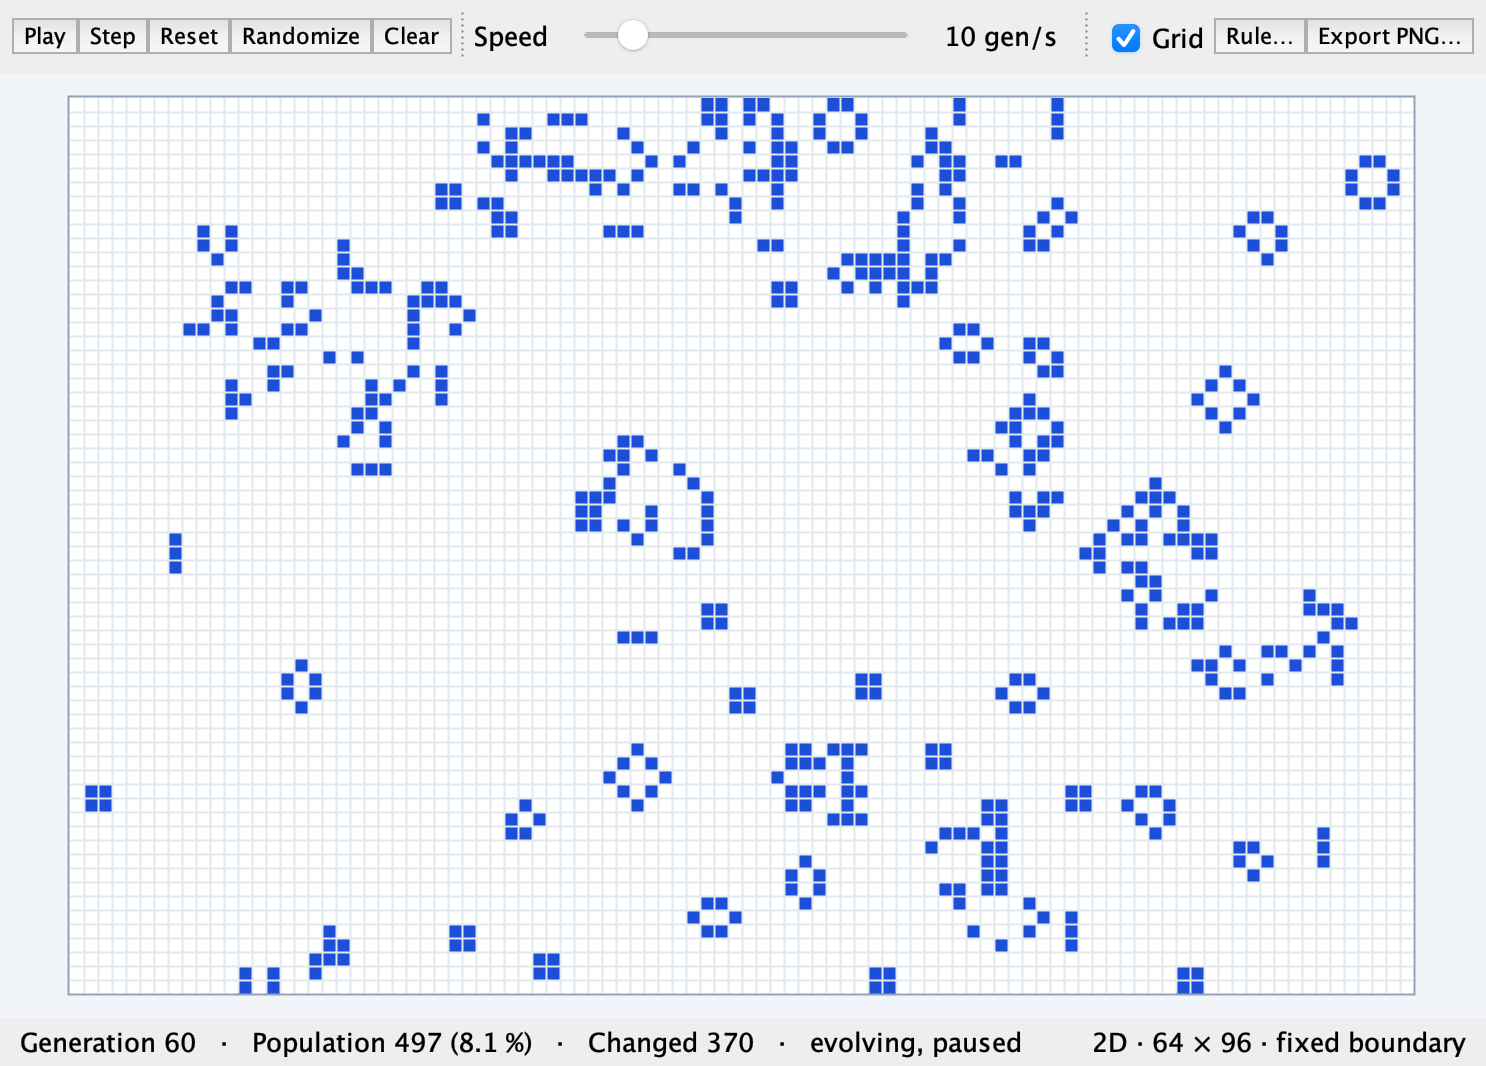
\includegraphics[width=\textwidth]{window-game-of-life}
    \caption{Game of Life, from \code{RANDOM(15)}}
  \end{subfigure}\hfill
  \begin{subfigure}[b]{0.46\textwidth}
    \centering
    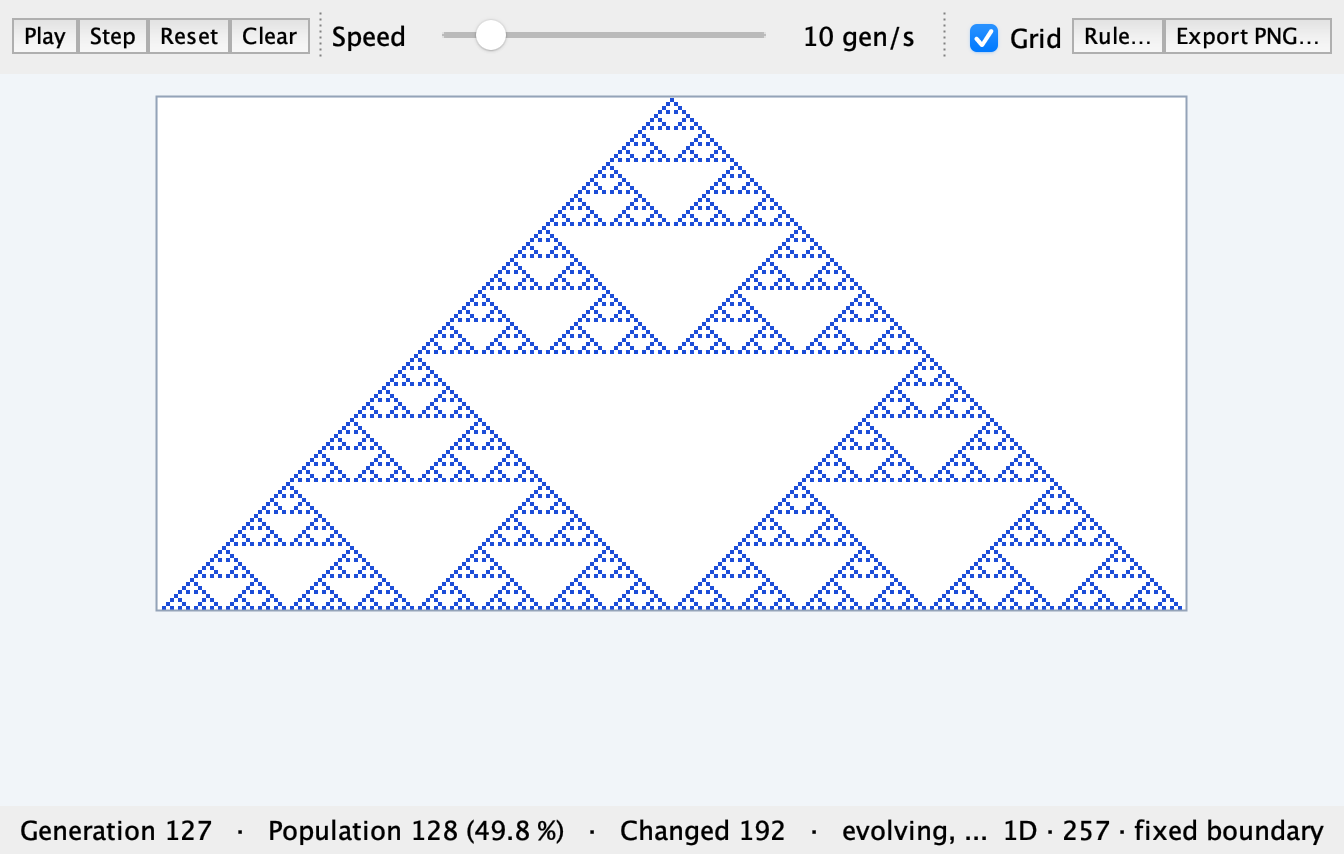
\includegraphics[width=\textwidth]{window-sierpinski}
    \caption{Sierpi\'nski triangle (rule 18)}
  \end{subfigure}
  \caption{The simulation window on the two definition files required by the subject.}
  \label{fig:teaser}
\end{figure}
